
%%%%%%%%%%%%%%%%%%%%%%%%%%%%%%%%%%%%%%%%%%%%%%
%--------- Symmetry --------------------------
%%%%%%%%%%%%%%%%%%%%%%%%%%%%%%%%%%%%%%%%%%%%%%



\chapter{Symmetry in crystallography}
\label{Chap:Symmetry}
Many objects in nature exhibit symmetry of some sort. The human body has approximate mirror symmetry. A shamrock (the species of clover or trefoil used as the symbol of Ireland) has three-fold rotational symmetry (trefoil), and here's a bit of trivia to make you a star at the next British party, not four-fold symmetry as U.S. advertisements sometimes wrongly represents it. The reader might have noticed that the way we talk about object symmetry involves a motion action, which made upon the object would leave it unchanged. Indeed, the symmetry of an object will be defined by its \textit{symmetry operations} that map the object onto itself. While for any motion one can find an object for which this is a  symmetry motion, if we start with the object it is easy to start with these three basic actions to test its symmetry\footnote{ Assuming we are to leave the metric properties of space undisturbed, \ie no stretching, bending, twisting, which should be easy to achieve in the physical world.}:
\begin{enumerate}
\item rotate
\item reflect
\item translate
\end{enumerate}

If, after any one or a combination of 1, 2 and 3, the object looks the same as it originally looked than we talk about the object as being symmetric. There is a nuanced distinction between these operations since 1 and 3 can be physically realised and known as \textit{proper} or first kind operations. Operations that involve 2 are \textit{improper} or of second kind. Inversion is yet another improper operation that can be reduced in three dimensions to a rotation plus a reflection. 

We will see that all this can be written in mathematical form with only minor adjustments. First, operation 3 can only truly be a symmetry operator for infinite objects which are not very common in everyday life. Second, the identity operator is also introduced as symmetry operator, such that, in the mathematical sense, all objects hold at least one symmetry property. Now there's nothing stopping you from being the soul of the party.

We will spend some time exploring a subset of symmetry operations chosen such that when combined can generate the entire symmetry of a wurtzite crystal. We will follow closely the notation used in \textit{International Tables for Crystallography, Volume A}~\cite{IntTableCrysA} described in some detail on page~\pageref{chap:int}. We will use the two most common shorthand notations to write down symmetry operations: the \textit{Hermann-Mauguin notation} also known as the \textit{international notation} which is the standard one, and the \textit{Schoenflies notation} which is widely used in Physics and Chemistry. We will also show the graphical symbols for the operations discussed.


\section{Symmetry operations}
\label{chap:symOp}
The set of symmetry operations of a given object have noteworthy properties:
\begin{enumerate}
\item the application of two symmetry operations results in a third symmetry operator of that object
\item the inverse of an operation is also an operation of that object
\item all objects exhibit the identity operation
\item the associative law is valid when combining three or more operations.
\end{enumerate}
These four properties are also the group axioms and tell us that the set of symmetry operations of a given object form a mathematical group. This will come in handy in the next section. For now it is worthwhile to look at how to write these operation in mathematical form.

In the following we will explore a non-exhaustive list of symmetry operations. We choose our examples such that they are relevant for generating the wurtzite crystal structure symmetry. Note that the  basis vectors of a hexagonal lattice do not form a Cartesian frame. This means that the usual algebraic formulas used for transformation operations must be revised. We do expect the form of rotation, translation and reflection matrices to be therefore not as familiar, which is why we take the time to explore them here. 



\subsection{Operation of first kind: pure rotation}
\label{sec:pureRot}

A pure rotation is fully determined by a rotation axis and a rotation angle which is chosen to be positive in the counter-clockwise direction. The rotation axis is given as a vector \hkl[uvw] and the rotation angle is given as fraction of $2\pi$. For instance a rotation of order three or three-fold rotation is a rotation by angle $2\pi/3$. In general an $n$-fold rotation is represented by symbol \textsf{n} (\textsf{C}$_n$) and Table~\ref{Table:rotation} shows examples for three-fold and six-fold rotations together with their graphical symbols which are filled polygons with $n$ sides.
 

\begin{table}[ht]
\caption{Examples of pure rotation symbols.}
\label{Table:rotation}
\centering
\begin{tabular}{l c c c }
\toprule
\tabhead{Name} & \tabhead{Graphical} & \tabhead{Hermann-Mauguin} & \tabhead{Schoenflies} \\
\midrule
 Three-fold rotation & {\Large \cry{3}} & \textsf{3} & \textsf{C$_3$} \\
 Six-fold rotation & {\Large \cry{6}} & \textsf{6} & \textsf{C$_6$}  \\
\bottomrule
\end{tabular}
\end{table}

\begin{figure}[ht]
    \centering
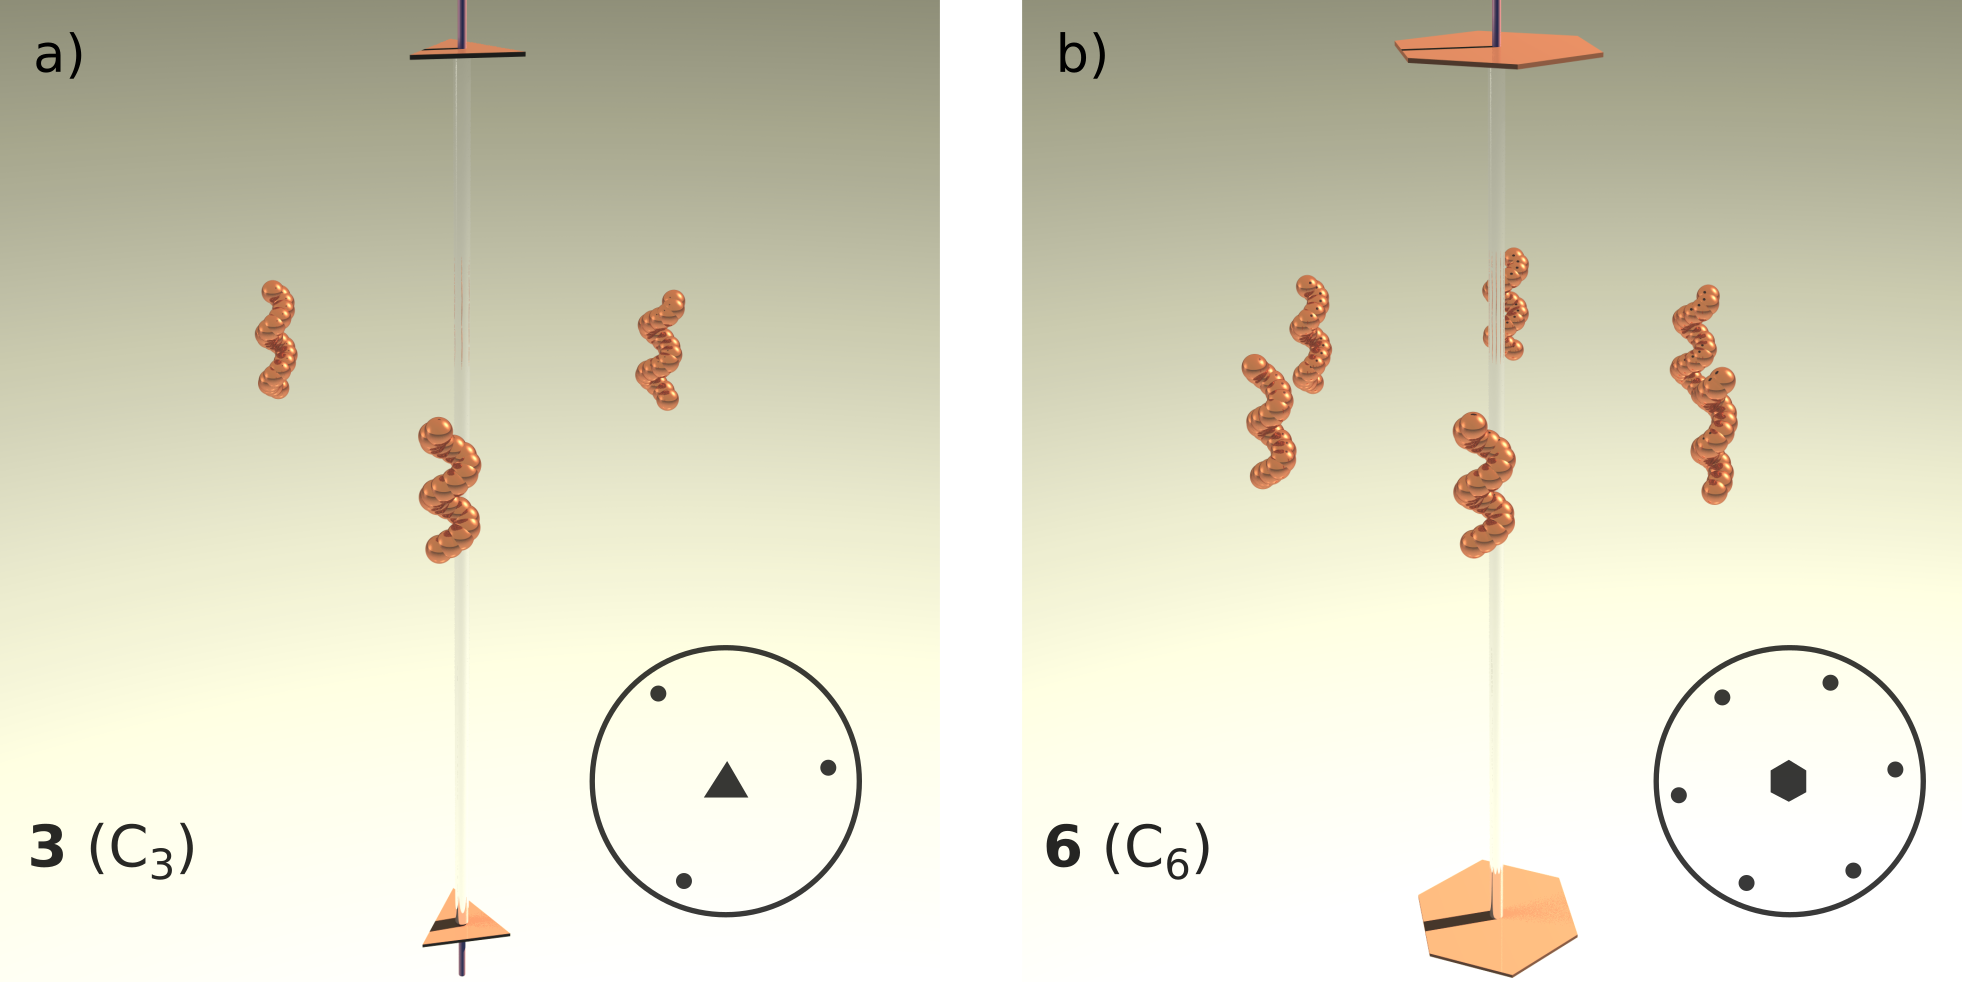
\includegraphics[width=0.9\linewidth]{Figures/pureRotation.png}
\caption[Graphical representations of three-fold and six-fold pure rotations.]{Rendered 3D graphical representations of a) three-fold and b) six-fold pure rotations. The circles in the bottom right of the images represent the stereographic projections of the operators.   }
\label{Fig:pureRotation}
\end{figure}

3D representations of the rotation operator are shown in Figure~\ref{Fig:pureRotation} for rotations of order 3 in (a) and 6 in (b), respectively. The images have been rendered with the public domain software \href{https://sourceforge.net/projects/rayshade/}{\textsf{Rayshade 4.0.9} software}\footnote{ Link is \href{https://sourceforge.net/projects/rayshade/}{https://sourceforge.net/projects/rayshade/}.}. The input files I used are very closely based on the input  \href{http://som.web.cmu.edu/frames2.html}{\emph{*.ray} files}\footnote{ Link is \href{http://som.web.cmu.edu/frames2.html.}{http://som.web.cmu.edu/frames2.html.}} developed by Marc De Graef~\cite{DeGraef98} with the purpose of teaching the crystallography group symmetry\cite{teachingPointGroup}. My scripts can be found at this \href{https://github.com/elena-pascal/SEM-diffraction/tree/master/Wurtzite_symmetry/}{GitHub repository}\footnote{ Link is \href{https://github.com/elena-pascal/SEM-diffraction/tree/master/Wurtzite_symmetry}{https://github.com/elena-pascal/SEM-diffraction/tree/master/Wurtzite\_symmetry}.}. The relevant files for this example are \texttt{3FoldPureRotationPNG.ray} and \texttt{6FoldPureRotationPNG.ray} and can be compiled on a Linux machine after the installation of \textsf{Rayshade} software (and making sure \textsf{ImageMagick} is available on the machine) by typing:
\begin{verbatim}
rayshade [filePNG].ray > [filePNG].mtv
convert [filePNG].mtv  [file].png 
\end{verbatim}
where \texttt{[file]} is the name of the file used. \emph{*.mtv} files can also be converted to \emph{*.png} or \emph{*.gif} with \textsf{ImageMagick}. All the input scripts and resulting images and animated files can be found in the extra materials. To render the \emph{*.gif}s one need more patience and has to do:
\begin{verbatim}
rayshade [fileGIF].ray > [fileGIF].mtv
convert [fileGIF].mtv  [file].gif 
\end{verbatim}

The small helix object used by Marc  De Graef in these images (made up of a helical string of spheres) was chosen such that it holds no rotational symmetry. The object also exhibits handedness and its mirror reflection will look different from the original object.  Despite this, the entire system, the three objects in Fig.~\ref{Fig:pureRotation} (a) or six objects in Fig.~\ref{Fig:pureRotation} (b), looks indistinguishable from original when rotated $2\pi/3 = 120\si{\degree}$ and $2\pi/6 = 60\si{\degree}$, respectively, around the rotation axis. Similarly, a triangle prism will look the same after being rotated around the central axis by $120\si{\degree}$ and a hexagonal prism will look indistinguishable after being rotated $60\si{\degree}$, respectively.

It is common for the axis of rotation to be the third basis vector \ie parallel to the crystallographic $\mathbf{c}$-axis and, in those cases, the rotation axis to not be explicitly stated. In any other case, the rotation axis must be given, either in vector form \hkl[uvw] or as the equation of the line coinciding with the axis. The latter notation method is the one used in the \textit{International Tables for Crystallography}. As an example we can look at \textit{Symmetry operation} (2) of a hexagonal lattice point group shown in Fig.~\ref{Fig:ITC}. $3^+(0,0,z)$ is a three-fold pure rotation around the \hkl[001] direction given here in line equation form. The $^+$~sign informs us that the position of the point is elevated with respect to the drawing plane. 

A three-fold symmetry of a lattice tells us that for every ``motif'' at position $(x, y, z)$ we will find the same motif at the equivalent position $(x', y', z')$ obtained through a $120\si{\degree}$ rotation around the central axis, here $\mathbf{e_z}$.  In order to represent the rotation operation in mathematical form we must turn to rotation matrices. Unlike the somewhat intuitive form when used in an everyday orthonormal system, as seen on page~\pageref{eq:RotMat}, when derived for a general, non-orthonormal lattice the rotation matrices can become cumbersome and will obscure the symmetry (see ref.~\cite{Davenport73}). Luckily, we can avoid that by considering the passive rotation of the system instead of the active rotation of the motif. 

We want to find the rotation matrix $\mathsf{D(}\theta\mathsf{)}$ which, when applied to a set of (not necessary orthonormal) basis vectors $(\mathbf{e_x},\, \mathbf{e_y},\, \mathbf{e_z})$ rotates them once around $\mathbf{e_z}$ by an angle $\theta$ to a new configuration $(\mathbf{e'_x},\, \mathbf{e'_y},\, \mathbf{e'_z})$. This passive rotation is defined in crystallography by the right hand rule\footnote{ The right thumb points towards the direction line and the fingers indicate the positive rotation.}. It should be clear that this is equivalent to an active rotation (\ie rotating a vector defined in this basis) by the same angle anticlockwise around $\mathbf{e_z}$ when looking in the direction of $\mathbf{e_z}$. 

\vspace{0.3cm}

\noindent \begin{minipage}{0.57\textwidth}

If the set of basis vectors describes a hexagonal lattice\footnotemark \, and the angle of rotation is $120\si{\degree}$ then the matrix $\mathsf{D^{hex}(120\si{\degree})}[001] \equiv \mathsf{D^{(n)}}$ is a three-fold rotation and can be derived by geometry as shown in Fig.~\ref{Fig:3foldrot}.
\begin{equation*}
\begin{split}
\begin{pmatrix}
\vb{e'_x} & \vb{e'_y} & \vb{e'_z}
\end{pmatrix}
 & =
\begin{pmatrix}
\vb{e_y} & -\vb{e_x} -\vb{e_y} & \vb{e_z}
\end{pmatrix} \\
&=\begin{pmatrix}
\vb{e_x} & \vb{e_y} & \vb{e_z}
\end{pmatrix}
\mathsf{D^{(n)}}
\end{split}
\end{equation*}

Which completely determines the matrix $\mathsf{D^{(n)}}$ to be:

\begin{equation}
\mathsf{D ^{(n)}} = \begin{pmatrix} 
0 & -1 & 0 \\
1 & -1 & 0 \\
0 & 0 & 1 
\end{pmatrix}
\label{eq:D_n}
\end{equation}
\end{minipage}
\begin{minipage}{0.4\textwidth}
    \centering
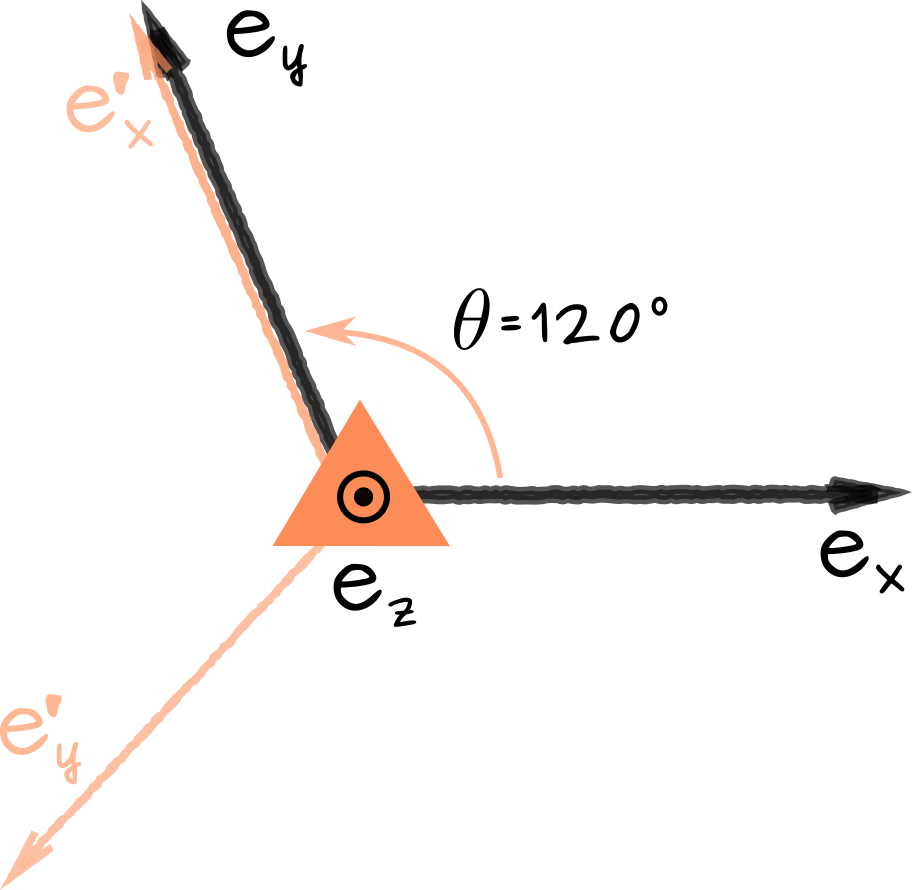
\includegraphics[width=0.85\linewidth]{Figures/3FoldaxisRot.png}
\captionsetup{width=0.7\linewidth}
\captionof{figure}{Three-fold rotation around the third axis of a hexagonal basis set. }
\label{Fig:3foldrot}
\end{minipage}

\vspace{0.5cm}

\footnotetext{ We have not explicitly shown that the hexagonal lattice is compatible with this symmetry operation but perhaps the reader will  not be too suspicious of a hexagon showing three fold rotation symmetry. }

It is not only rotations that can be expressed in matrix form, reflections as well as any combination of reflection and rotation can be written down as matrix operations. Every possible symmetry operation a crystal holds, if it excludes translation, will be part of a finite and well determined group of 3$\times$3 matrices. Only a subset of these matrices is really necessary to determine the entire group and these are known as \textit{generators}. There are only 14 matrices $\mathsf{D^{(x)}}$ that can act as generators, where $\mathrm{(x)}$ spans from $\mathrm{(a)}$ to~$\mathrm{(n)}$. Talking in detail about groups and space groups is beyond the purpose of this thesis, but a good introduction to crystallography for the electron microscopist can be found in \textit{Structure of Materials; an introduction to crystallography, diffraction and symmetry}~\cite{SoM} while an in-depth overview is given in the introduction to the \textit{ International Tables for Crystallography, Volume A}~\cite{IntTableCrysA} both of which we will reference throughout this section.

\subsection{Operation of first kind: pure translation}
A pure translation is fully determined by translation vector $\vb{t}=u_1\vb{e_1} + u_2\vb{e_2} + u_3\vb{e_3}$. The lattice translation vector was introduced on page~\pageref{Sect:spaceLattice} and to it we can be add the lattice centring vectors if present. The latter are useful for describing non-primitive lattices where lattice points exists not only at the corners of the crystal structure. The international symbol for translation is t($u_1$, $u_2$, $u_3$) as can be observed in the representation of the basis vectors given in the \textit{Generators} list in Fig.~\ref{Fig:ITC}: t($1$,~$0$,~$0$), t(0,~1,~0), t(0,~0,~1).

Mathematically, a translation is just a vector addition:
\begin{equation}
\vb{r'} = \vb{r} + \vb{t}.
\label{eq:translation1}
\end{equation}
However, we want to integrate this into the matrix formulation we developed for the rotation operation. To achieve this we introduce a 4D vector. By adding a trivial equation in the form of a fourth component which is just: $1$ $(x_1, x_2, x_3) \rightarrow (x_1, x_2, x_3, 1)$. We also upgrade the Einstein notation to go from $i=1$ to $i=4$, such that Eq.~\ref{eq:translation1} becomes: $x'_i =x_i + u_i$ or in matrix form:

\begin{equation}
\begin{pmatrix}
x'_1\\
x'_2\\
x'_3\\
1\\
\end{pmatrix}
=
\begin{pmatrix}
1 & 0 & 0 & u_1 \\
0 & 1 & 0 & u_2 \\
0 & 0 & 1 & u_3 \\
0 & 0 & 0 & 1
\end{pmatrix}
\begin{pmatrix}
x_1\\
x_2\\
x_3\\
1\\
\end{pmatrix}
\label{eq:w_ex}
\end{equation}

The $4\times4$ matrix consists of the $3\times3$ rotation matrix $\mathsf{D^{(i)}_{ij}}$ in the upper left corner, a $3\times1$ column vector containing the translation vector components on the right and a $1\times4$ row at the bottom, $(0 \, 0\, 0\, 1)$, containing no useful information. We will introduce the symbol $\mathcalboondox{W}$ for the $4\times4$ matrix such that: 
\begin{equation*}
x'_i=\mathcalboondox{W}_{ij} x_j.
\end{equation*}

\label{eq:Seitz}
In practice, it is more useful to denote the rotation matrix and translation vector that are implied, which is why the \textit{Seitz symbol}, written as $(\mathsf{D} |\vb{t})$, is more commonly used. For instance, the $\mathcalboondox{W}$ matrix in Eq.~\ref{eq:w_ex} has the Seitz symbol $(\mathsf{E} |\vb{t})$, where $\mathsf{E}$ is the identity matrix $\mathsf{D}$. The $\mathcalboondox{W}$ matrix for a rotation plus translation is:

\begin{equation}
\label{eq:Wdef}
\mathcalboondox{W} = (\mathsf{D} |\vb{t}) = 
\begin{pmatrix}
\mathsf{D_{11}} & \mathsf{D_{12}} & \mathsf{D_{13}} & u_1 \\
\mathsf{D_{21}} & \mathsf{D_{22}} & \mathsf{D_{23}} & u_2 \\
\mathsf{D_{31}} & \mathsf{D_{32}} & \mathsf{D_{33}} & u_3 \\
0 & 0 & 0 & 1 \\
\end{pmatrix}.
\end{equation}
   
The pure rotation in Eq.~\ref{eq:D_n} has the Seitz symbol $(\mathsf{D^{(n)}} |\vb{0})$ and as a $4\times4$ matrix becomes:

\begin{equation*}
\mathcalboondox{W}_\text{\cry{3}} = 
\begin{pmatrix}
0 & -1 & 0 & 0 \\
1 & -1 & 0 & 0 \\
0 & 0 & 1 & 0 \\
0 & 0 & 0 & 1 \\
\end{pmatrix}.
\end{equation*}

   
\subsection{Operation of second kind: pure reflection}
\label{sec:pureRefl}
A pure reflection operation, more commonly known as a \textit{mirror}, is characterised by the reflection plane. When it does not coincide with the plane of drawing, the mirror plane is  schematically indicated by a solid line, as shown in Table~\ref{Table:mirror}. The international notation for mirror plane provides also information on the orientation of the plane, usually by writing down the equation of the plane. For instance, the mirror plane parallel to \hkl(110) is written as $m(x,\, -x,\, z)$. We can find this symmetry operation at number (7) on page 584 of the \textit{Tables}, shown in Fig.~\ref{Fig:ITC}.


\begin{table}[ht]
\caption{Example of pure reflection symbols.}
\label{Table:mirror}
\centering
\begin{tabular}{l c c c }
\toprule
\tabhead{Name} & \tabhead{Graphical} & \tabhead{Hermann-Mauguin} & \tabhead{Schoenflies} \\
\midrule
 Mirror plane & \rule[1pt]{0.5in}{2pt} & \textsf{m} & ${\sigma}$ \\
\bottomrule
\end{tabular}
\end{table}
   
   
\noindent\begin{minipage}{0.57\textwidth}
Mirror operations can be represented by a matrix $\mathsf{D}(m)$, which, analogous to the rotation matrix, can be determined from geometry. For the reflection operation in Fig.~\ref{Fig:mirrorplane}:
\begin{equation*}
\begin{split}
\begin{pmatrix}
\vb{e'_x} & \vb{e'_y} & \vb{e'_z}
\end{pmatrix}
 & =
\begin{pmatrix}
-\vb{e_y} & -\vb{e_x} & \vb{e_z}
\end{pmatrix} \\
&=\begin{pmatrix}
\vb{e_x} & \vb{e_y} & \vb{e_z}
\end{pmatrix}
\mathsf{D}(m)
\end{split}
\end{equation*}
From which we find the set operation $\mathsf{D}^{hex}(m_{(x,-x,z)})\equiv \mathsf{D^{(k)}}$ to be:

\begin{equation}
\mathsf{D^{(k)}} = \begin{pmatrix}
0 & -1 & 0 \\
-1 & 0 & 0 \\
0 & 0 & 1 
\end{pmatrix}.
\label{eq:D_k}
\end{equation}

\end{minipage}
\begin{minipage}{0.4\textwidth}
    \centering
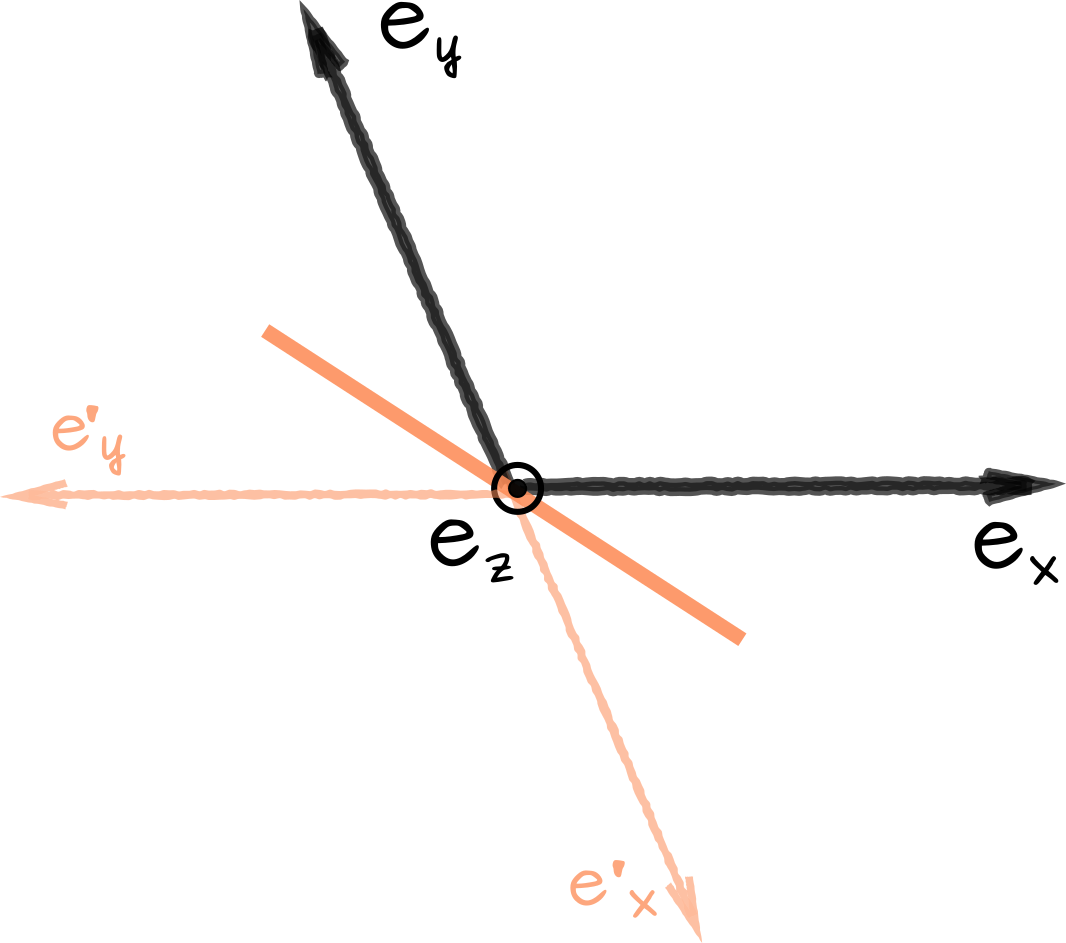
\includegraphics[width=0.9\linewidth]{Figures/mirrorPlane.png}
\captionsetup{width=0.7\linewidth}
\captionof{figure}{ $m(x,\, -x,\, z)$ mirror plane operation in a hexagonal basis set. }
\label{Fig:mirrorplane}
\end{minipage}

\vspace{0.2cm}
Which, in turn, completely determines the matrix $\mathcalboondox{W}_\mathsf{m}$ with Seitz symbol  $(\mathsf{D^{(k)}} |\vb{0})$.



\subsection{Combination of rotation and translation}
\label{sec:screw}
Combining translation with rotation yields a new type of symmetry operation, known as a \textit{screw axis}. While applying a pure rotation of order $n$ to an object we recover the original position after $n$ successive operations, the extra translation operation in the screw axis renders this observation invalid. During a screw axis operation, the object is translated after every rotation step by a certain vector $\boldsymbol{\tau}$ parallel to the rotation axis. We can see that in Fig.~\ref{Fig:ScrewRotation}. Input files used are \texttt{2\_1PNG.ray} and \texttt{6\_1PNG.ray}  (see how to use them in the \textit{Pure Rotation} subsection on page~\pageref{Fig:pureRotation} ).  For a $\mathsf{2_1}$ screw axis shown in Fig.~\ref{Fig:ScrewRotation} a), after a two-fold ($2\pi/2=180\si{\degree}$) rotation, the object is also translated by a vector $\boldsymbol{\tau}$ from point~\textbf{0} to point~\textbf{1}. After $n=2$ rotations it is translated $2 \boldsymbol{\tau}$ in the direction of the screw axis to the point~\textbf{2}. This position is identical to the original one except for a translation vector $m \vb{t}$ where $\vb{t}$ is the smallest possible translation vector in the given direction and, in this case, $m=1$. This is where the subscript $_\mathsf{1}$ comes from in the notation $\mathsf{2_1}$.


\begin{figure}[ht]
    \centering
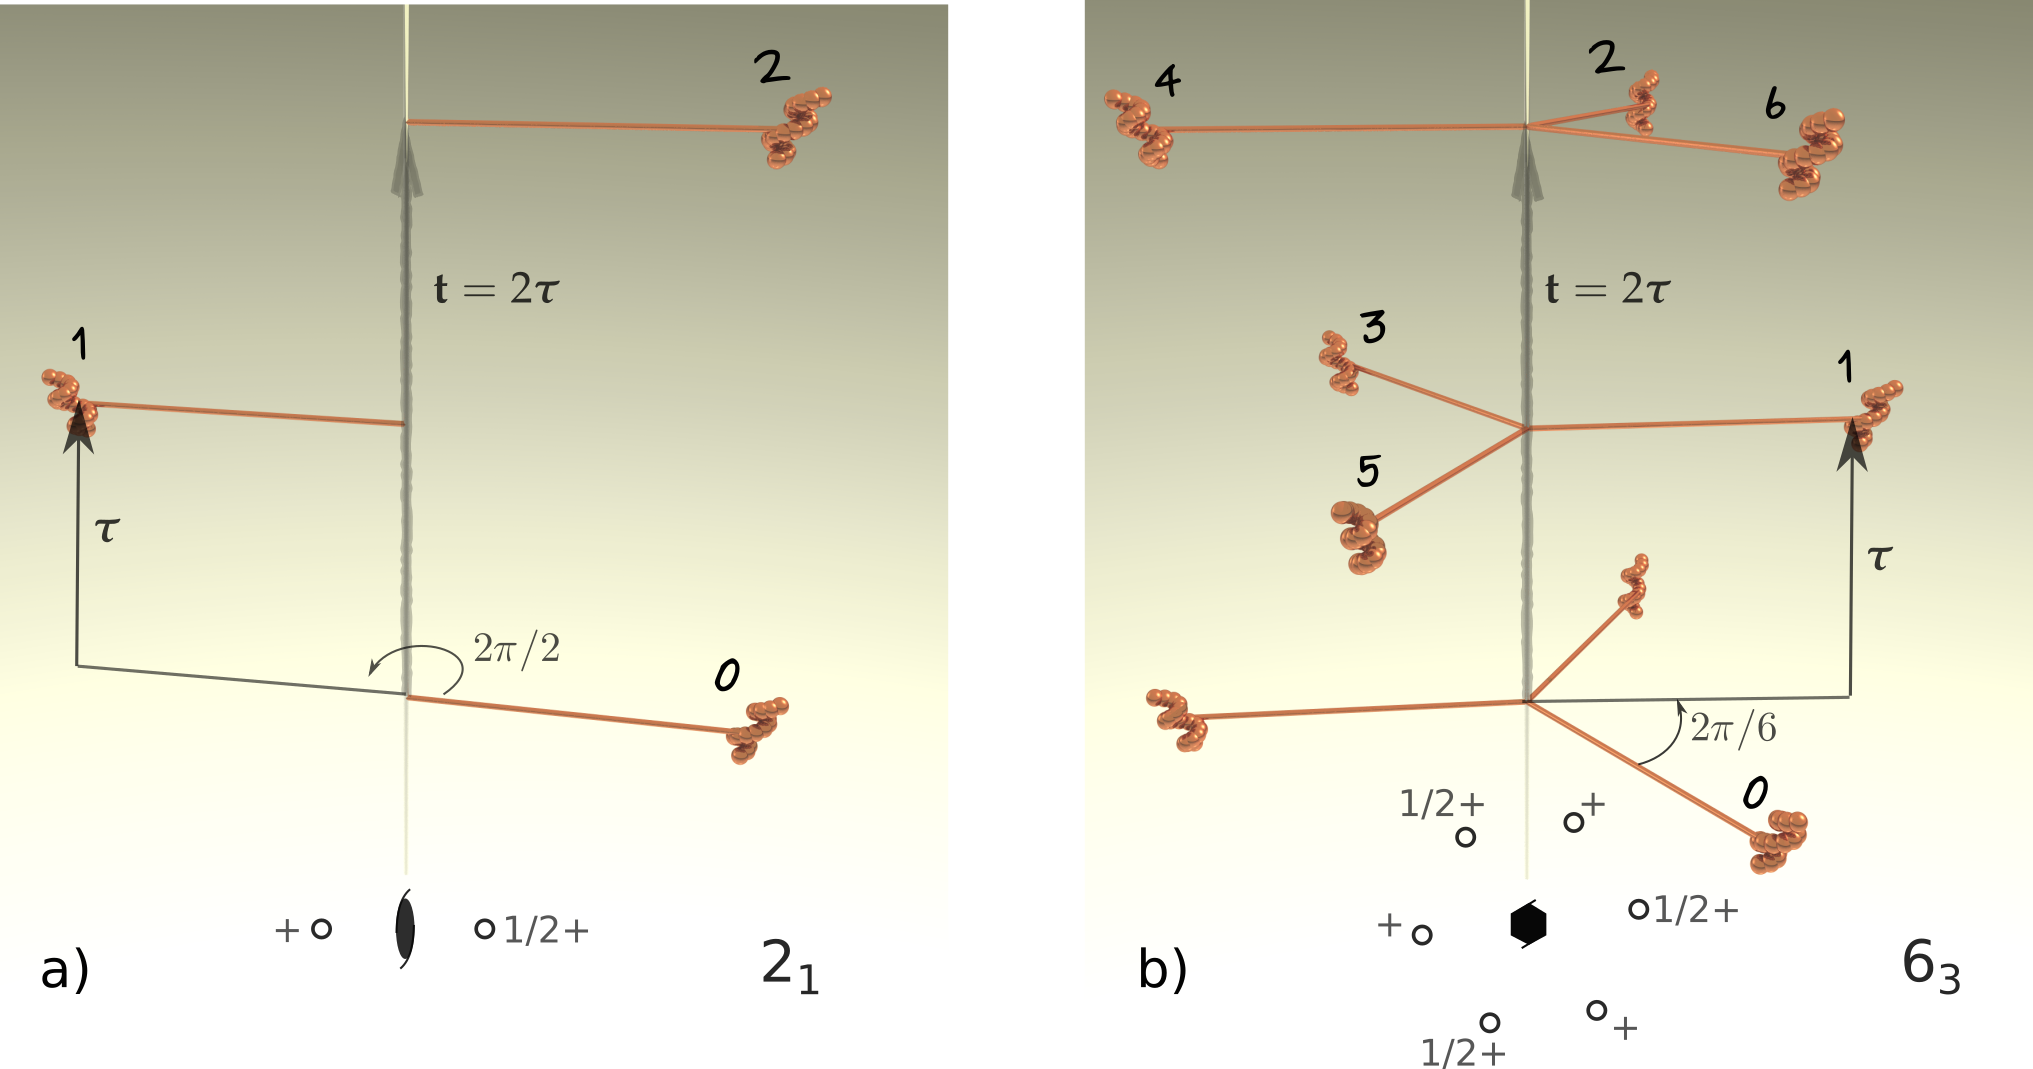
\includegraphics[width=1.\linewidth]{Figures/screwRotation.png}
\caption[Operations steps for screw axis.]{Rendered 3D graphical representations and (sequentially numbered) operations involved in the construction of screw axis a)~$\mathsf{2_1}$ and b)~$\mathsf{6_3}$. Standard 2D graphical projections are included at the bottom. }
\label{Fig:ScrewRotation}
\end{figure}

Generally, the notation for a screw axis is $\mathsf{n_m}$ where $n\boldsymbol{\tau} = m\vb{t}$, which tells us that after $n$ screw axis operations the original point is translated $m$ lattice translation vectors in the direction of the screw axis. One screw axis operation involves an $n$-fold rotation plus a $\boldsymbol{\tau}=m\vb{t}/n$ translation. Table~\ref{Table:screwAxis} shows the graphical and notation symbols for the relevant screw axis operations of the wurtzite crystal:  $\mathsf{2_1}$ and $\mathsf{6_3}$.  The $\mathsf{6_3}$ operation, shown in Fig.~\ref{Fig:ScrewRotation} b), involves a $\boldsymbol{\tau} = 3\vb{t}/6=\vb{t}/2$ translation after each six-fold rotation, which takes the object on which it operates from point \textbf{0} to point \textbf{1}. After two $\mathsf{6_3}$ operations the object has been translated by a total vector equal to the lattice translation vector $\vb{t}$. To obtain the next points, \textbf{3}, \textbf{4} and \textbf{6}, we must leave the unit cell in which we started. Because all unit cells must be the same, the screw rotation in the cell below dictates equivalent points in this cell corresponding to the position of points \textbf{3}-\textbf{6}.

The bottom of the images in Fig.~\ref{Fig:ScrewRotation} contain standard graphical representation of the corresponding symmetry operations such that the axes of rotation are normal to the page. The open circles indicate that the objects are above the plane of drawing and the numbers next to the circle refer to the height of their positions. 


\begin{table}[ht]
\caption{Examples of screw axis symbols.}
\label{Table:screwAxis}
\centering
\begin{tabular}{l c c c }
\toprule
\tabhead{Name} & \tabhead{Graphical} & \tabhead{Printed} & \tabhead{Screw vector $\boldsymbol{\tau}$ in units of $\vb{t}$} \\
\midrule
 Two-fold screw axis & {\Large \cry{21}} & $\mathsf{2_1}$ & $1/2$ \\
 Six-fold screw axis & {\Large \cry{63}} & $\mathsf{6_3}$ & $1/2$  \\
\bottomrule
\end{tabular}
\end{table}

The \textit{International Tables for Crystallography} denote the screw axis operations by the order of the rotation together with the translation vector $\boldsymbol{\tau}$: $n(\boldsymbol{\tau})$. The axis of rotation is also added as it can be seen in the symmetry operations list on page~\pageref{Fig:ITC}. Operation (4), for instance, denotes a  $\mathsf{2_1}$ screw axis around the $\vb{c}$-axis in a hexagonal unit cell. 
\vspace{0.3cm}

\noindent \begin{minipage}{0.57\textwidth}

Mathematically, we can write this operation from geometry (see Fig.~\ref{Fig:screwOperation}) as:
\begin{equation*}
\begin{split}
\begin{pmatrix}
\vb{e'_x} & \vb{e'_y} & \vb{e'_z}
\end{pmatrix}
 & =
\begin{pmatrix}
-\vb{e_x} & -\vb{e_y} & \vb{e_z}
\end{pmatrix} \\
&=\begin{pmatrix}
\vb{e_x} & \vb{e_y} & \vb{e_z}
\end{pmatrix}
\mathsf{D^{(b)}}
\end{split}
\end{equation*}

From which we find the set operation $\mathsf{D^{(b)}}$ to be:
\begin{equation}
\mathsf{D^{(b)}} = \begin{pmatrix} 
-1 & 0 & 0\\
0 & -1 & 0 \\
0 & 0 & 1 
\end{pmatrix} .
\label{eq:D_b}
\end{equation}

\end{minipage}
\begin{minipage}{0.4\textwidth}
\vspace{0.3cm}
    \centering
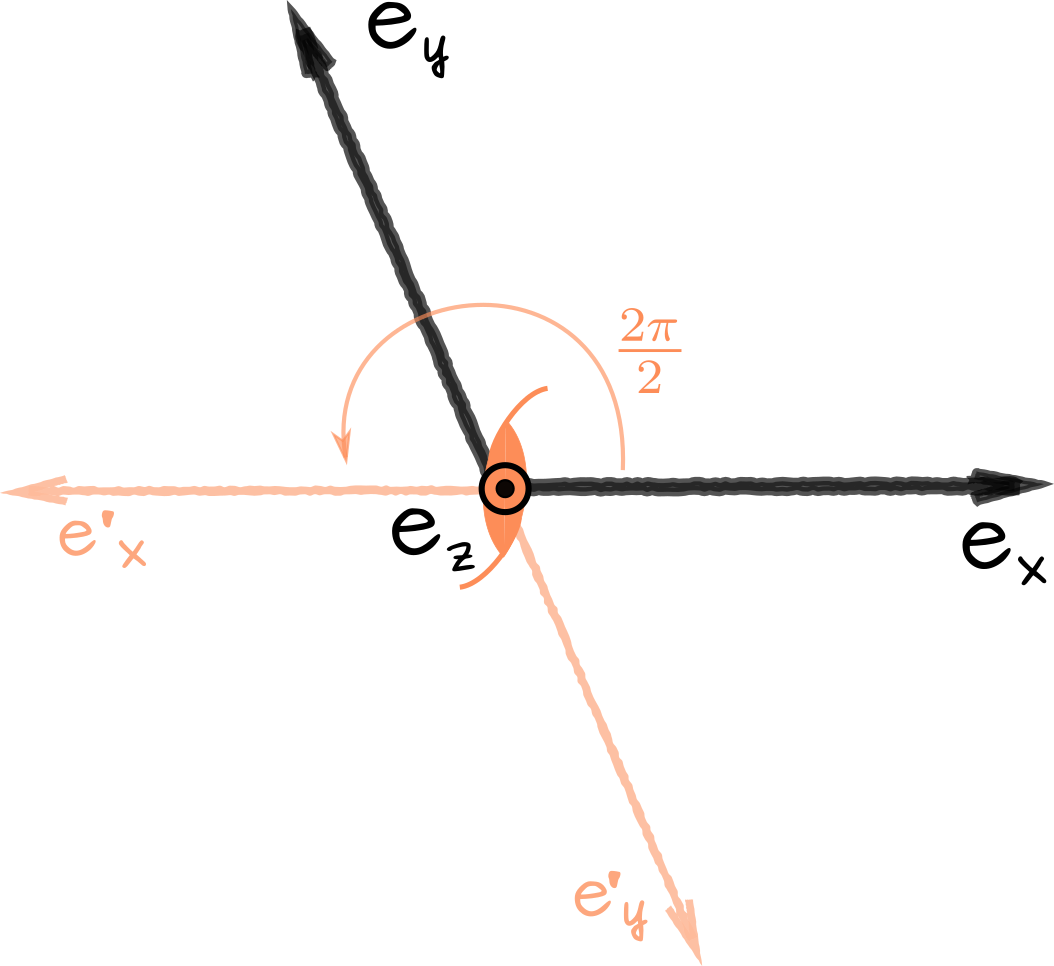
\includegraphics[width=0.9\linewidth]{Figures/screw2.png}
\captionsetup{width=0.7\linewidth}
\captionof{figure}{ $\mathsf{2_1}$ screw axis operation in a hexagonal basis set. }
\label{Fig:screwOperation}
\end{minipage}


\vspace{0.5cm}
 Which completely determines the matrix $\mathcalboondox{W}_\text{\cry{21}}$ with Seitz symbol  $(\mathsf{D^{(b)}} |\boldsymbol{\tau}_{(0,\, 0,\, 1/2)})$:


\begin{equation*}
\mathcalboondox{W}_\text{\cry{21}} = \begin{pmatrix} 
-1 & 0 & 0 & 0\\
0 & -1 & 0 & 0\\
0 & 0 & 1 & 1/2 \\
0 & 0 & 0 & 1
\end{pmatrix} .
\label{eq:21screwW}
\end{equation*}
Now that we have written out the mathematical framework necessary for studying a number of different symmetries we can take a closer look at how to describe a crystal structure starting from the symmetry it manifests. More importantly, we want to answer the question ``\textit{What is the minimum number of symmetry operations from which a specific structure can be recovered?}''.   



%======================================================================
%==============================Point groups============================
%======================================================================

\section{Point groups}

It turns out maths already has the answer to that question and it can easily be applied to crystallography. If we forget for a moment about translations, then any of the remaining symmetry operators can be applied to an object and leave exactly one point invariant, namely the origin. For all the symmetry operations we talked about, the choice of the origin (a plane for reflection, an axis for rotation~\dots) was non-ambiguous. Another way of saying this is that all symmetry operators except translation overlap in exactly one point. All these operators can be expressed as $3 \times 3 $ matrices $\mathsf{D}$ and carry the name of \textit{point symmetries}. The total point symmetries of an object must also form a \textit{group} with the properties given on page~\pageref{chap:symOp}. If the object under consideration is a crystal structure, then those symmetry operations are selected such that they are compatible with the translational periodicity of its lattice. Starting, then, from a \textit{point} one can derive 32 sets of consistent symmetry operations compatible with the Bravais lattices also known as crystallographic point groups (see Chapter 9 in~\cite{SoM}).

Groups have several useful properties, including the fact that one can generate all elements of a group starting with a list of operations and constructing a multiplication table. The minimum symmetry operations needed to construct a full point group is known as a set of \textit{generators}. There are only 14 total generators, a subset of which will produce any possible crystal symmetry. We have encountered three of them so far, denoted as  $\mathsf{D^{(b)}}$,  $\mathsf{D^{(k)}}$ and $\mathsf{D^{(n)}}$. The matrices $\mathsf{D^{(i)}}$ form the set of generators where $(i)$ can go from $(a)$ to $(n)$, $\mathsf{D^{(a)}}$ being the identity matrix, which, as previously discussed, describes the symmetry of all systems and is always implied.


We keep on following the Hermann-Mauguin and Schoenflies notations for crystallographic point groups, with the latter shown in brackets. The Hermann-Mauguin notation for point groups has a maximum of three symbols, each corresponding to a particular direction in the Bravais lattice. Since the choice of origin is very specific when we consider the possible symmetries a crystal would exhibit, the possible axes of symmetry for a given crystal will be the directions used to describe the point group of a particular system. 

Table~\ref{Table:symdirections} shows the three directions for the three possible set of symbols describing the point group of a hexagonal crystal system. For instance, we can consider a group made up of only the identity operation and all powers\footnote{ An operator to power 2 simply means applying that operator twice in succession.} of the rotation operator, we talked about rotation operations on page~\pageref{sec:pureRot}. The notation of this simple group will follow the notation of the operators, therefore, a six-fold rotational point group (also known as cyclic) is $\mathbf{6}$ or $\mathbf{C_6}$ (C for cyclic).\footnote{ Note that we use the Sans Serif font for operators symbols and the Bold font for group notation.} If a hexagonal crystal is known to be part of the crystallographic point group $\mathsf{6}$ then we can conclude it has six-fold rotational symmetry and can read from Table~\ref{Table:symdirections} that the rotation axis must be \hkl[00.1].


\begin{table}[ht]
\caption[Symmetry directions for the hexagonal crystal.]{Primary, secondary and tertiary symmetry directions (Miller-Bravais) for the hexagonal crystal.}
\label{Table:symdirections}
\centering
\begin{tabular}{l c c c }
\toprule
\tabhead{Crystal system} & \tabhead{Primary\hkl[uv.w]} & \tabhead{Secondary\hkl[uv.w]} & \tabhead{Tertiary\hkl[uv.w]} \\
\midrule
 Hexagonal & \hkl[00.1]& \hkl{10.0} & \hkl{12.0} \\
\bottomrule
\end{tabular}
\end{table}

Now that we set the rules with the simplest of examples let's take a look at something a bit more involved. \textit{(1) What happens if we combine the proper rotation group with reflection operations? and (2) How do we generate the full symmetry of such a group?} 

\subsection{\texorpdfstring{$\mathbf{6mm}$}{6mm} point group from generators}
\label{subChap:pointGroup}
If we give a mirror plane ($\mathsf{m}$) a six-fold rotation axis ($\mathsf{6}$) then we end up with the point group shown in Fig.~\ref{Fig:6mm}. Notice the change of handedness (chirality) of the orange object as an indication of the reflection symmetry. The generating file is \texttt{6mmPNG.ray}. It turns out that, for even rotation orders, an extra mirror symmetry appears. One can easily see that in the stereographic projection at the bottom of the image. Every second mirror is not generated by the rotation operation, however the structure clearly displays the extra reflections. This is why the group $\mathbf{6mm}$ has two `$\mathsf{m}$'s in its notation. From Table~\ref{Table:symdirections} we can read that the first set of mirrors have the normals \hkl{10.0} while the second set of mirrors have the normals \hkl{12.0}. Similarly, the $_\mathbf{v}$ in the Schoenflies notation $\mathbf{C_{6v}}$ indicates the vertical orientation of the mirror planes.  

\begin{figure}[ht]
    \centering
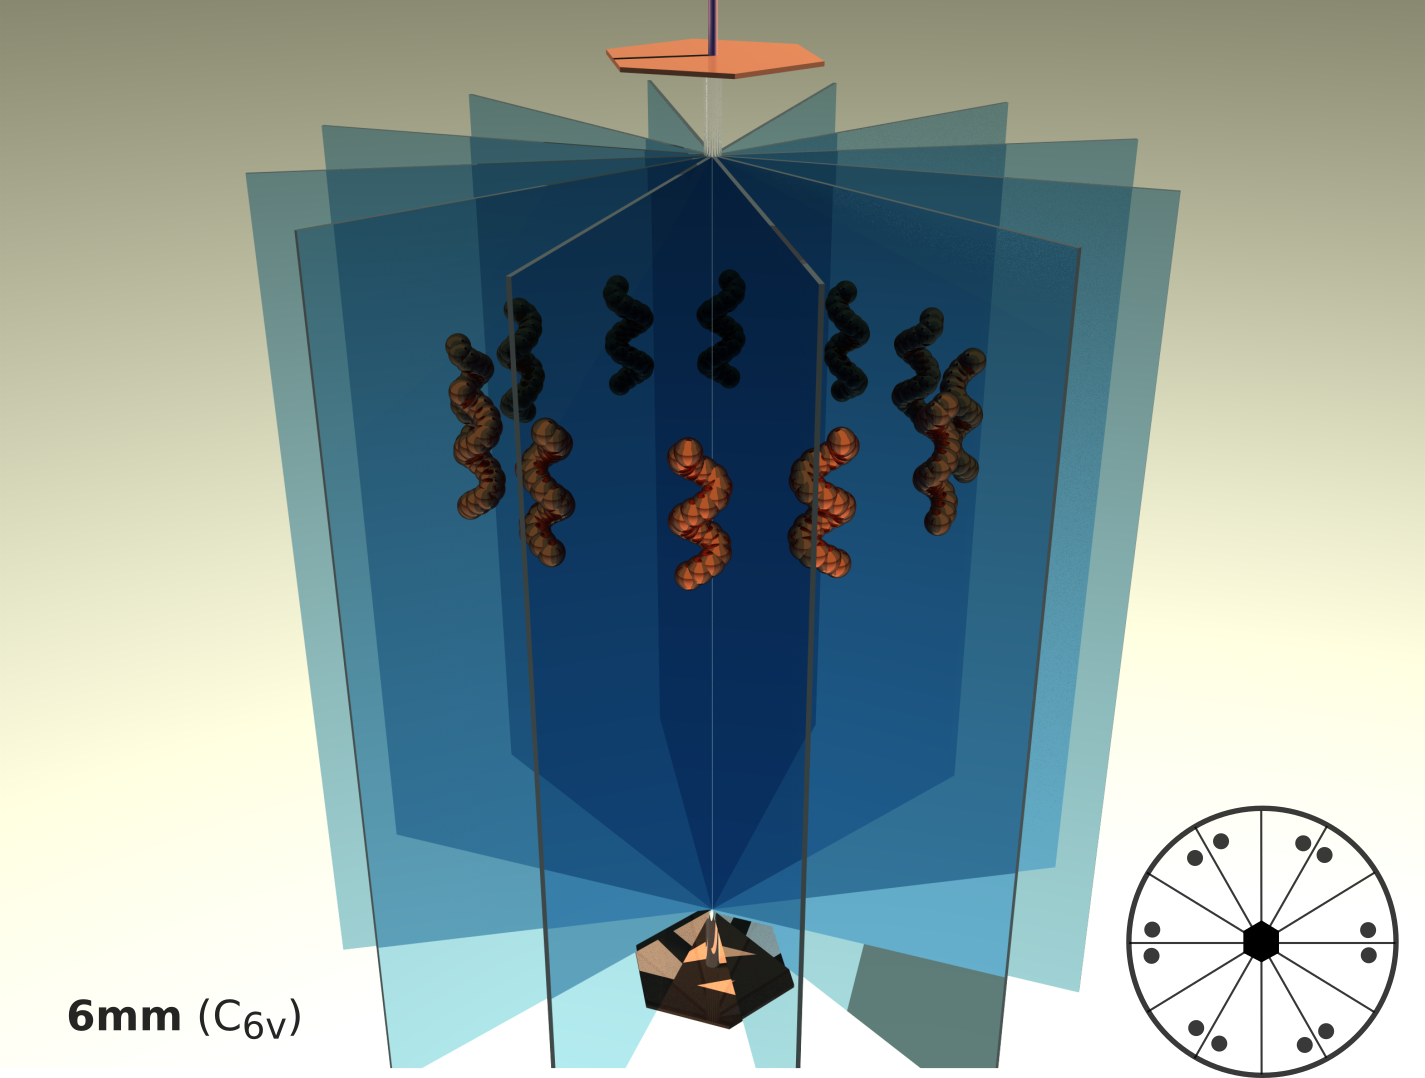
\includegraphics[width=0.85\linewidth]{Figures/pointGroup.png}
\caption[ $\mathbf{6mm}$ point group. ]{ Graphical 3D representation of $\mathbf{6mm}$ point group together with its stereographic projection in the bottom corner right. }
\label{Fig:6mm}
\end{figure}




The generators matrices of $\mathbf{6mm}$ point group are: $\mathsf{D^{(a)}}$,  $\mathsf{D^{(b)}}$, $\mathsf{D^{(k)}}$, $\mathsf{D^{(n)}}$; where we denoted the identity operator with the label $\mathsf{D^{(a)}}$. Conveniently, we have already derived the three $3\times3$ matrices corresponding to the last three of these operators: $\mathsf{D^{(b)}}$ (Eq.~\ref{eq:D_b}), $\mathsf{D^{(k)}}$ (Eq.~\ref{eq:D_k}), $\mathsf{D^{(n)}}$ (Eq.~\ref{eq:D_n}). We can find these matrices in the \textit{International Tables for Crystallography, Volume A}~\cite{IntTableCrysA} in the \textit{Generators} list of the space group (pages 584-585 shown here on page~\pageref{Fig:ITC}) as operations $(1)$, $(2)$, $(4)$, $(7)$. In order to find the full list of symmetry operators of the space group, we can read the \textit{Symmetry operations} section from the \textit{Tables} or we can multiply the generators among themselves until we find the full list of 12. We'll show here the hard way for the reader to use as a reference but also to somewhat demystify the origin of these matrices.


Before that we want to add a few notes on point group characteristics. The number 12 represents the size of the set of points in this group which have equivalent position. That is to say, if we start with an arbitrary position $(x, y, z)$ how many new positions are generated when the full set of symmetry operations are applied. This is also known as the \textit{order} of the group. We can then say that the $\mathbf{6mm}$ point group has order 12. 
Another point group property is that of \textit{centrosymmetry}.  If we define polarity as the property of a group in which directions $\vb{t}$ and $\vb{-t}$ are not related to each other by any symmetry operation, then we can note that this group is only polar along the rotation axis. We can also conclude that this point group is not centrosymmetric.


To find the full symmetry of a point group starting with the list of generator matrices, we multiply each operator with itself and the others, remembering that matrix multiplication is not commutative. For every resulting matrix that is not the identity matrix we check if we already have it in the set. If not then we can add it and start the matrix multiplications again. When we did all the possible operations in a set without finding any new matrices we can stop looking and declare we found the full symmetry operations group. The \emph{Python} style pseudocode for this is shown below in Algorithm~\ref{Fc:symMatrices}. This function is implemented in the Jupyter notebook \texttt{Symmetry\_matrices.ipynb}. 

\begin{algorithm}[ht]
\caption{Recursive function to find the symmetry matrices of a space group starting from the list of generators. }
\DontPrintSemicolon
\SetKwProg{Fn}{def}{\string:}{end}
\SetKwFunction{findsymmatrices}{findSymMat}
\SetKwData{isThisNew}{isThisNew}
\SetKwData{knownMat}{knownMat}
\SetKwData{newMat}{newMat}
\SetKwInOut{Input}{input}\SetKwInOut{Output}{output}

\Fn{\findsymmatrices{\knownMat, *\newMat}}{
\Input{List of $3 \times 3$ generator matrices}
\Output{Entire list of symmetry operators as $3 \times 3$ matrices }
\BlankLine
\While{still finding new matrices}{
\BlankLine
\For{matrix\_i in \newMat}{
	\For{matrix\_j in \knownMat}{
		\BlankLine
		\isThisNew = $matrix\_i$ $\times$ $matrix\_j$ \;
			
		\BlankLine
		\uIf{\isThisNew is not Identity Matrix and is not in \knownMat}{
			add \isThisNew to \newMat \;
			add \isThisNew to \knownMat \;}
		\Else{stop looking}		
	}
}
\BlankLine
\If{new matrix is found}{
	\findsymmatrices(\knownMat, \newMat)
}

}
}

\label{Fc:symMatrices}
\end{algorithm}

\vspace{0.2cm}

Using this implementation%
\footnote{ Luckily, there is a good selection of mature or novel open software available to do these type of computations as well. Here are a few examples:
\begin{itemize}
\item \href{www.gap-system.org}{GAP} - provides an extensive computational group theory algebra library and tools.
\item \href{http://docs.mantidproject.org/v3.7.1/concepts/PointAndSpaceGroups.html}{Mantid} - available as a \textit{Python} package, can handle crystallographic point and space group maths.
\item \href{https://atztogo.github.io/spglib/python-spglib.html}{spglib} - another \textit{Python} package, can do symmetry computations. 
\item \href{https://github.com/marcdegraef/EMsoft}{EMsoft} - the routine \texttt{CalcPositions} in the module \texttt{symmetry.f90} should do a generalised version of the implementation shown here.
\end{itemize}
}
 we find the following 12 symmetry matrices of the $\mathbf{6mm}$ point group: $\mathsf{D^{(a)}}$, $\mathsf{D^{(b)}}$, $\mathsf{D^{(k)}}$, $\mathsf{D^{(n)}}$, $\mathsf{D^{(nn)}}$, $\mathsf{D^{(nb)}}$, $\mathsf{D^{(nk)}}$, $\mathsf{D^{(kn)}}$, $\mathsf{D^{(kb)}}$,  $\mathsf{D^{(bnk)}}$, $\mathsf{D^{(nkk)}}$, $\mathsf{D^{(knk)}}$ (not necessary in the same order as in the \textit{Tables}). Here we used the notation: $\mathsf{D^{(nb)}} = \mathsf{D^{(n)}} \times \mathsf{D^{(b)}}$ to represent a combination of operations applied in a specific order. For instance, $\mathsf{D^{(nn)}}$ is a 3-fold rotation applied twice and it should come as no surprise that a 3-fold rotation applied tree times is the identity operator: $\mathsf{D^{(nnn)}} = \mathsf{D^{(a)}}$. Similarly, $\mathsf{D^{(kk)}}$ is a double reflection and, again, equals to the identity operator.

The equivalent positions in the space group can then be easily determined by simply applying these operators to a general position $(x, y, z)$.



\section{Space groups }

So far we have explored some possible symmetries of a system (motif) that are compatible with the hexagonal Bravais lattice of a crystal structure. It is time to add these point group symmetries to the crystal lattice points and observe what new symmetries emerge. This simply involves combining the point group operators with the Bravais lattice translational vectors of a given crystal system. Every time this combination yields a new unique system then we can talk about a different symmetry group this time known as a \textit{space group}. 

There are 230 three dimensional space groups which might sound like a formidable result when we considered that we only combine 32 point groups with 14 Bravais lattices. However, bear in mind that there are more than one way of adding the point group symmetries at the lattice points. Additionally, combining symmetry operation can yield extra symmetries, just like the extra mirror planes ``popped up'' in the $\mathsf{6mm}$ point group. Screw axes and glide planes\footnote{ We haven't explicitly talked about glide planes, but these are symmetry operations obtained by combining a mirror plane with translation over half the lattice vector parallel to the mirror plane. The symbol for a glide plane is $a$, $b$ or $c$ if the glide vector is $\vb{a}/2$, $\vb{b}/2$ or $\vb{c}/2$, respectively.} are symmetry operators containing a translation vector and therefore not forming point groups. However, when used to point group symmetries, in combination with Bravais lattices, these operators will form new space groups. 

The space group symbol is formed by combining the centring information of the Bravais lattice with the point group Hermann-Mauguin notation symbol. The information about the symmetry of the crystal system can be dropped since it will be implied in the point group symmetry. One can predict extra symmetry operations describing a unique space group by replacing one or more operations in the Hermann-Mauguin point group notation with a screw rotation or glide plane. It is entirely possible to end up with a situation in which the point group of a space group contains operations which do not occur in the space group at all.  
 
Depending on whether or not the space group contains any glide planes or screw axis symmetry operations we differentiate between \textit{non-symmorphic} and \textit{symmorphic} space groups. Symmorphic space groups contain then only the point group operations and are easy to spot from their Hermann-Mauguin symbols.






 


%%
\subsection{The \textit{International Tables for Crystallography, Volume A}}
\label{chap:int}

The series of volumes constituting the \textit{International Tables for Crystallography} are a comprehensive database of crystallographic information relevant in the studies of the structure or properties of materials. \textit{Volume A}~\cite{IntTableCrysA}, specifically tackles the space groups. We have already referenced a few times to a specific page in \textit{Volume A} which shows all the information needed for the study of the space group symmetry $\mathbf{P6_3mc}$ in tabulated form. It is a useful skill for a crystallographer to be able to read these pages.

\begin{itemize}  
 \item The top of the page holds the crystal system (hexagonal), the Patterson symmetry definition\footnote{ The Patterson function is a mathematical construct of higher symmetry than the electron density function which it replaces in order to  solve the phase problem in X-ray crystallography. }, the point group symmetry (6mm), the Schoenflies symbol (\textsf{C$^4_{6v}$}), the complete space group symbol ($P6_3mc$), the space group shorthand symbol $\mathbf{P6_3mc}$ and the space group number (186).
 
 \item Below, there is a drawing of the relative positions of the symmetry elements in the group, projected along the main direction ($\mathbf{c}$), on the right. On the left, the equivalent positions are shown in the same projection.
 
 \item While the \textit{Origin} of the group can be chosen arbitrarily, it is customary to choose the position with the highest symmetry of the group; here $6_3mc$\footnote{ Note that, while the notation is point group like, the origin position symmetries do not need to form a group and we do not keep the point group symbol notation.}. The symmetry is given in the usual point group notation following the system's symmetry directions (seen in Table~\ref{Table:symdirections}). To clarify the ambiguity a second set of symmetries is given $3m1$, where the $1$ is a place-holder for no more than identity symmetry for this direction, to establish the origin in the upper left corner of the unit cell.
 
 \item The \textit{Asymmetric unit} is the smallest volume of the unit cell that will completely and exactly fill the space when the group's symmetry operators are applied to it. It is defined in terms of the sides and vertices containing the volume, which in turn are the result of the intersecting symmetry planes bounding the cell. The volume of the asymmetric cell has the property of being the volume of the full unit cell divided by the product of the order of the point group, $n$, (for $\mathsf{6mm}$ $n=12$ ) and the number of centring operations plus one. For $\mathbf{P6_3mc}$ then, the volume of the asymmetric cell is $V_a = V/(12 \times 1)=V/12$.
 
 \item Below, the full list of \textit{Symmetry operations} together with their positions is given and we have already shown how to read some of these operations. There are a total of 12 symmetry operators including the identity  operator.
 
 \item From these operators only 4 make it to the list of \textit{Generators}, (1), (2), (4), and (7), together with the basis translation vectors. Starting with these list of 4 operators the full previous list can be generated by matrix multiplication.
 
\begin{figure}
    \centering
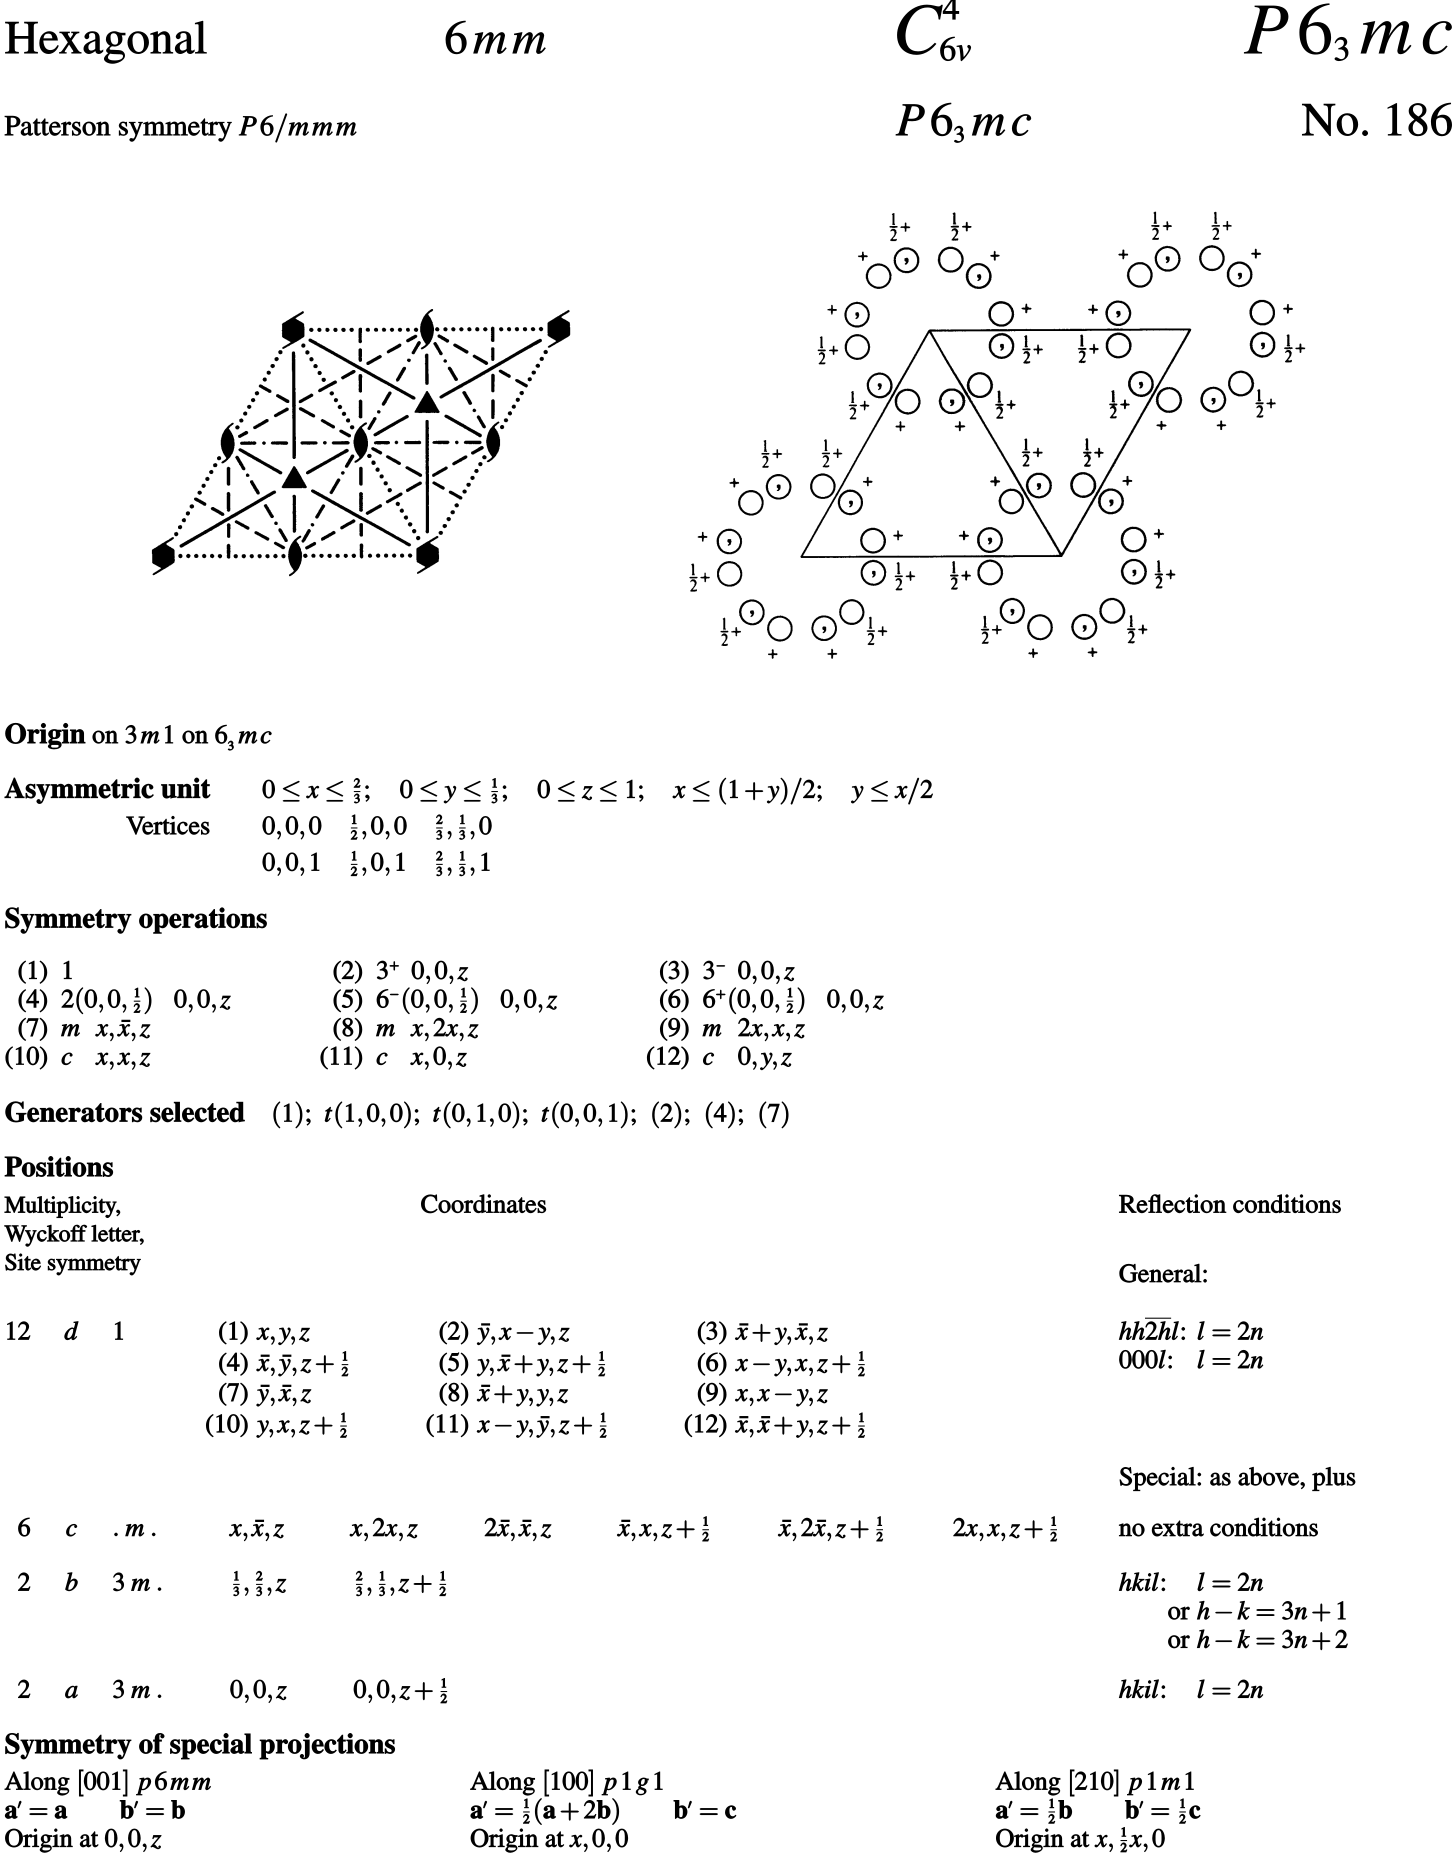
\includegraphics[width=1.\linewidth]{Figures/ITC.png}
\caption[Space group $\mathbf{P6_3mc}$ in \textit{ITC}]{ Pages 584-585 (compressed here) of \textit{International Tables for Crystallography, Volume~A}~\cite{IntTableCrysA} describing the space group $\mathbf{P6_3mc}$. }
\label{Fig:ITC}
\end{figure}

 \item The \textit{Position} tables contain the symmetrically equivalent points in the crystal system divided between the general positions in the first block followed by the special positions blocks underneath. The general position is left invariant by the identity operator but no other symmetry operation of the space group, while the special positions are left invariant by at least one other symmetry operation in addition to the identity. All the symmetry operations that map a point onto itself form together a \textit{site symmetry }group for that position given in the third column of the table. The coordinates for the general position,  ($i$)$x', y', z'$,  are the result of a symmetry operation ($i$) on the most general position $x, y, z$. These can also be viewed as a shorthand notation of the symmetry matrices of the group. The numbers in the first column indicate the number of equivalent points per unit cell or the \textit{multiplicity} of the position. For the general position the multiplicity is the number of symmetry operators, while for the special positions each added site symmetry reduces the multiplicity by the order of symmetry. For instance, the second positions entry shows a mirror site symmetry which halves the multiplicity of the point to 6.  The \textit{Wyckoff letters} are labels for the Wyckoff positions, which in turn are a way of describing the positions of the atoms in the asymmetric unit. The last column in this table, entitled \textit{reflection conditions}, is a list of diffraction information given as requirements for the structure factor to not be zero (conditions of occurrence) for the given position. 
 
 \item The last section shown here is the \textit{Symmetry of special projections} which contains two dimensional projection information of the unit cell along lattice directions. If the wurtzite unit cell is projected along the \hkl[100] direction, then the resulting 2D object will have $\mathbf{p6mm}$ plane group symmetry and will be defined by the unit vectors $\mathbf{a'}$ and $\mathbf{b'}$ which in general are expected to be fractions of linear combinations of the original basis vectors. The origin of the 2D unit cell is also specified.  
\end{itemize}

 
An account of crystal symmetry would be incomplete without referencing the \textit{International Tables for Crystallography}. Now that we know how to read the \textit{Tables} we can just read out the results of many of the derivations we have done in this Appendix. 
